\RequirePackage{luatex85}
\documentclass[9pt,aspectratio=169]{beamer}

\usepackage[all]{xy}
\usepackage{luamplib}
\everymplib{input mpcolornames; beginfig(1);}
\everyendmplib{endfig;}

\usetheme{graham}

\title{Arithmetic sequencies}
\subtitle[Graham Middle School]{Graham Middle School Math Olympiad Team}

\begin{document}
\maketitle

\begin{frame}{Gaussian sums}
  \begin{columns}[T]
    \begin{column}{0.5\textwidth}
      To keep his 3\textsuperscript{rd} grade students busy, a teacher in 18th century Germany asked to find the sum of the numbers from $1$ to $100$. But one of the students in the class was 10-year-old Carl Friedrich Gauss.  He instantly answered $5050$.

      How did he do that?  To sum the digits 
      \[ \xymatrix@C=-2pt@R=0pt{
        1\ar@/_/[dddrrrrr] & + & 2\ar@/_/[ddrrr] & + & 3\ar@/_/[dr] & +\ \ldots\ + & 98\ar@/^/[dl] & + & 99\ar@/^/[ddlll] & + & 100\ar@/^/[dddlllll] \\
        & & & & & 101 & & & & & \\
        & & & & & 101 & & & & & \\
        & & & & & 101 & & & & & 
      } \]
      we pair terms as shown. So total, we have $50$
      \begin{wrapfigure}{r}{0.7\textwidth}
        \vspace*{-1.3em}
        \hspace*{-1em}
        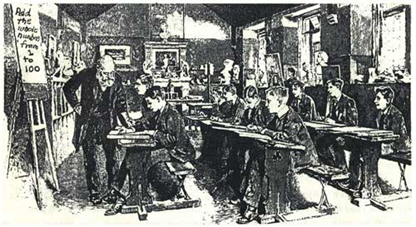
\includegraphics[width=0.8\textwidth]{06 - Arithmetic Sequences/school.png}
      \end{wrapfigure}
      pairs~with 
      a~value~$101$. 
      Then multiplying them together, we will get $5050$.
    \end{column}
    \begin{column}{0.5\textwidth}
      \begin{problem}
        What is the sum of first $n$ numbers?
      \end{problem}
      If n is even, there are $\dfrac{n}{2}$ pairs, each equal to $n+1$, and the sum is $\dfrac{n \left(n + 1\right)}{2}$.  
      
      If $n$ is odd, the middle term, which is equal to $\dfrac{n + 1}{2}$, is unpaired, and there are $\dfrac{n − 1}{2}$ paired terms that each sum to $n + 1$.  So in the odd case the total sum is $\dfrac{n + 1}{2} + \dfrac{\left(n-1\right)\left(n+1\right)}{2}$ which also equals $\dfrac{n \left(n + 1\right)}{2}$. 
      \begin{definition}
        The sum of the counting numbers from $1$ to $n$ is equal to $\dfrac{n \left(n + 1\right)}{2}$. 
      \end{definition}
      This formula is easy to remember as $n$ is the number of terms, and $\left(n + 1\right) / 2$ is the average or arithmetic mean value of the terms in the series.
    \end{column}
  \end{columns}
\end{frame}

\begin{frame}{Arithmetic sequences}
  \begin{columns}[T]
    \begin{column}{0.5\textwidth}
      \begin{definition}
        An \textbf{arithmetic sequence} is a sequence of numbers in which \emph{consecutive terms} differ by the \textbf{same amount}.
      \end{definition}
      For example
      \[ 5,\ 11,\ 17,\ 23,\ 29,\ 35,\ 41. \]
      An order of elements in a sequence matters.The sequence $1$, $2$, $3$, $4$ is not the same as the sequence $4$, $3$, $2$, $1$. 

      Arithmetic sequences are sometimes referred to as \textbf{arithmetic progressions}, and terms that form an arithmetic sequence are said to be "in arithmetic progression." For example $7$, $9$, $11$, $13$ are in arithmetic progression.
      
      Sequence can also have \emph{infinitely} many terms. For example \emph{counting numbers} are \emph{infinite arithmetic sequence}
      \[ 1,\ 2,\ 3,\ 4,\ 5,\ 6,\ 7,\ 8,\ 9,\ 10,\ 11,\ 12,\ \ldots \]
    \end{column}
    \begin{column}{0.5\textwidth}
      \begin{definition}
        In an arithmetic progression, the \emph{first number} in the series is called the \textbf{initial (first) term}.\smallskip

        The value by which \emph{consecutive terms increase or decrease} is called the \textbf{common difference}.
      \end{definition}
      Usually initial term denoted as $a$ or $a_1$ and common difference as $d$.

      Some examples
      \[
        \begin{array}{l r r}
          \text{arithmetic sequence}\hspace*{3em} & a_1 & \hspace*{2em}d \\
          1,\ 2,\ 3,\ 4,\ 5,\ 6,\ \ldots & 1 & 1 \\
          5.5,\ 7.8,\ 10.1,\ 12.4,\ \ldots & 5.5 & 2.3 \\
          4,\ 2,\ 0,\ -2,\ -4,\ -6,\ \ldots & 4 & -2 \\[0.4em]
          \dfrac{2}{3},\ \dfrac{5}{6},\ 1,\ \dfrac{7}{6},\ \dfrac{4}{3},\ \ldots & \dfrac{2}{3} & \dfrac{1}{6} \\[0.7em]
          x,\ 2x,\ 3x,\ 4x,\ 5x,\ \ldots & x & x
        \end{array}
      \]
      \begin{center}
        \vspace*{-1\baselineskip}
        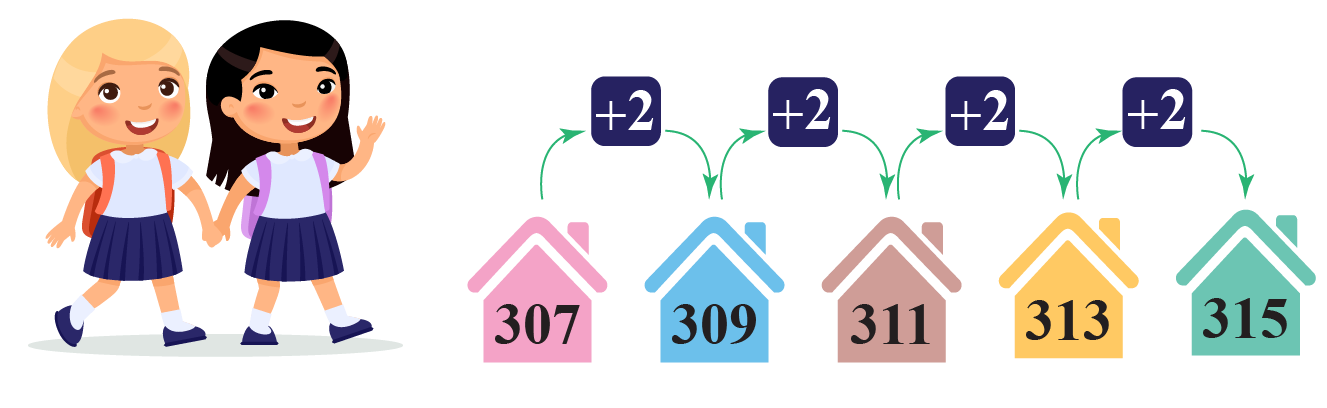
\includegraphics[width=0.9\textwidth]{06 - Arithmetic Sequences/street.png}
      \end{center}
    \end{column}
  \end{columns}
\end{frame}

\begin{frame}{General term of arithmetic sequence}
  \begin{columns}[T]
    \begin{column}{0.5\textwidth}
      \begin{problem}
        On February 1\textsuperscript{st}, Alice starts reading a book and ends on page $10$ (she read the forward and introduction). Then she reads $3$ pages per day. How many pages will she read by February 15\textsuperscript{th}?
      \end{problem}
      She will read $3$ pages for $14$ days (from February 2\textsuperscript{nd} till February 15\textsuperscript{th}), so she will read total of 
      \[ 3 \times 14 = 42 \]
      pages after February 1\textsuperscript{st}. So total she will read 
      \[ 42 + 10 = 52 \]
      pages.
      \begin{wrapfigure}{r}{0.5\textwidth}
        \vspace*{-2.5em}
        
\includegraphics[width=0.5\textwidth]{06 - Arithmetic Sequences/reading.jpg}
      \end{wrapfigure}
      The number of pages she has read by the end of the day from an arithmetic sequence
      \[ 10,\ 13,\ 16,\ 19,\ 21,\ \ldots \]
      And 15\textsuperscript{th} term of this sequence is $52$.
    \end{column}
    \begin{column}{0.5\textwidth}
      \begin{problem}
        An initial term of an arithmetic series is $a$, and a common difference is $d$. Find a term on $n$\textsuperscript{th} place?
      \end{problem}

      The second term is the initial term and the common difference, the third term is the second term plus the common difference, and so on.
      \begin{multline*}        
        \text{Term} = \text{Initial Term} + {} \\ {} + \left(\text{Common Difference} \times \hspace*{7em}\right. \\ \left.{} \times \text{Number of steps from the initial term}\right).
      \end{multline*}
      Or written as a formula for a general term of an arithmetic sequence:
      \begin{definition}
        \[ a_n = a_1 + d \times (n - 1). \]
        \vspace*{-0.5\baselineskip}
      \end{definition}
      It is also worth mentioning, each term in the arithmetic series is an average of its neighbors.
    \end{column}
  \end{columns}
\end{frame}

\begin{frame}{Arithmetic series}
  \begin{columns}[T]
    \begin{column}{0.5\textwidth}
      \begin{definition}
        The \emph{sum} of the terms of an arithmetic sequence is called an \textbf{arithmetic series}.
      \end{definition}
      \begin{problem}
        Find the sum $7 + 11 + 15 + 19 + \ldots + 83 + 87$?
      \end{problem}

      Let's do the trick done by Gauss in 3\textsuperscript{rd} grade. We pair numbers: $7$ with $87$, $11$ with $83$, $15$ with $79$, and so on. Each pair has the sum $94$, and we just need to find a total number of pairs.\smallskip

      \emph{How to know how many terms we have?}

      To get from $7$ to $87$ we need to add $4$ $20$ times, which means that we have a total of $21$ terms.

      That means we have $10$ pairs and one element in the middle of the sequence. The element is on 11\textsuperscript{th} place, so it should be equal to 
      \[ 7 + 4 \times (11 – 1) = 47. \]
      The sum of the arithmetic series is 
      \[ 94 \times 10 + 47 = 987. \]
    \end{column}
    \begin{column}{0.5\textwidth}
      \begin{definition}
        The \textbf{number of terms} in the arithmetic series is
        \[ \frac{\text{last term} - \text{first term}}{\text{increment}} + 1.\]
        \vspace*{-0.8em}
      \end{definition}
      Instead of using elements in pairs, we can replace both terms with $2$ average values. This will not change the sum, but all terms will become the same. 
      \begin{definition}
        In an arithmetic series, the \textbf{average value} is 
        \[ \frac{\text{first term} + \text{last term}}{2}. \]\vspace*{-0.8em}
      \end{definition}
      This will leads us to formula for a sum of arithmetic series.
      \begin{definition}
        In an arithmetic series, the sum is 
        \[ \text{average value} \times \text{number of terms}.\]\vspace*{-1.2em}
      \end{definition}
    \end{column}
  \end{columns}
\end{frame}

\begin{frame}{Repeating geometric pattern}
  \begin{columns}[T]
    \begin{column}{0.5\textwidth}
      A popular variety of question in middle school math contests involves series of geometric patterns.  Consider this question from MOEMS in December 2020:
      \begin{problem}
        \hspace*{0.7em}
        \begin{mplibcode}
          u=0.25cm;
          s=0.63cm;
          numeric shift;
          path v;
          path h;      
          shift:=0;    
          for i = 1 upto 4:
            shift:=shift + s + i*u;
            %fill (u + shift, 0)--(u + u*i + shift, 0)--(u + u*i + shift, -1*u)--(u + shift, -1*u)--(u + shift, 0);
            v := (u + shift, 0)--(u + u*i + shift, 0)--(u + u*i + shift, -1*(2+i)*u)--(u+shift, -1*(2+i)*u)--cycle;
            h := (shift, -u)--(shift + (2+i)*u, -u)--(shift + (2+i)*u, -1*(1+i)*u)--(shift, -1*(1+i)*u)--cycle;
            fill v withcolor 0.78;
            fill h withcolor 0.78;
            fill (u + shift, -1*u)--((1+i)*u + shift, -1*u)--((1+i)*u + shift, -1*(1 +i)*u)--(u+shift, -1*(1+i)*u)--cycle withcolor 0.96;
            draw v;
            draw h;
            for j = 1 upto i-1:
              draw (j * u + u + shift, 0)--(j * u + u + shift, -u);
              draw (j * u + u + shift, -1*(1 +i)*u)--(j * u + u + shift, -1*(2 +i)*u);
              draw (shift, -1* j * u - u)--(shift + u, -1* j * u - u);
              draw ((1+i)*u + shift, -1* j * u - u)--((2+i)*u + shift, -1* j * u - u);
            endfor
          endfor
          pickup pencircle scaled 3pt;
          shift:=shift + s + 5*u;
          drawdot (shift, -3*u);
          shift:=shift + u/1.5;
          drawdot (shift, -3*u);
          shift:=shift + u/1.5;
          drawdot (shift, -3*u);
        \end{mplibcode}

        Each figure in the sequence shown is composed entirely of $1 \times 1$ shaded squares.  If the pattern is continued, how many $1 \times 1$ shaded squares will there be altogether in the first $21$ figures?
      \end{problem}
    \end{column}
    \begin{column}{0.5\textwidth}
      There are $4$ squares in the first figure, $8$ squares in the second figure, $12$ squares in the third figure and so on.

      With each successive figure, they are adding one square to each side, and there are $4$ sides, so the number of squares for the $n$\textsuperscript{th} figure in the series is $4n$.  So we have figured out the pattern, and now have the general expression for the value of any term in this arithmetic series.

      The total number of squares in the first $21$ figures
      \[ 4 + 8 + 12 + \ldots + 84 = 4 \left(1 + 2 + 3 + \ldots + 21\right). \]
      Using Gauss' rule for summing integers from $1$ 
      to~$n$, the sum of the integers $1$ to $21$ is:
      \[ \frac{22 \times 21}{2} = 231. \]
      The total number of squares is $4 \times 231 = 924.$

    \end{column}
  \end{columns}
\end{frame}

\begin{frame}{Arithmetic series shortcuts}
  \begin{columns}[T]
    \begin{column}{0.5\textwidth}
      You don't always need to use a formula to calculate the sum of arithmetic series.
      \begin{problem}
        Find the sum of the sequence: $7 + 8 + \ldots + 106$?
      \end{problem}
      When we replace $101$ with $1$, $102$ with $2$, and so on until $106$ with $6$ we will get the sum of the first $100$ consecutive integers. The result must be the sum of the numbers from $1$ to $100$ ($= 5050$) plus $600$ for a total of $5650$.  The $600$ is added because the first $6$ terms of the series have been reduced to get the example that Gauss summed.
      \begin{problem}
        Consider the arithmetic series 
        \[ 7,\ 14,\ 21,\ \ldots,\ 693,\ 700. \]
        What is the sum of the elements in the series?
      \end{problem}
      We may see that each element in this series is seven times larger than the numbers $1-100$, so this sum must be $7 \times$ larger than $5050$. Well, 
      \[ 7 \times 5050 = 35350. \]
    \end{column}
    \begin{column}{0.5\textwidth}
      The sums of arithmetic series are usually denoted as $S_n$, where $n$ is the number of terms.

      It is also helpful to know some sums that are often used in olympiad problems.
      \begin{definition}
        Sums of arithmetic series of \emph{counting numbers} $1$, $2$, $3$, $4$, $\ldots$ are called the \textbf{triangular numbers}.
      \end{definition}
      \begin{wrapfigure}{r}{0.15\textwidth}
        \begin{mplibcode}
          u=0.5cm;
          h=sqrt(3)/2;
          draw (0,0)--(3u, 0);
          draw (u, 2u*h)--(2u, 2u*h); 
          draw (0.5u, u*h)--(2.5u, u*h); 
          pickup pencircle scaled 6pt;
          for i=0 upto 3:
            for j=0 upto i: 
              drawdot (i*u - j/2*u, j*u*h) withcolor VioletRed3; 
            endfor
          endfor
        \end{mplibcode}
      \end{wrapfigure}
      \vspace*{-0.6\baselineskip}
      \begin{align*}
        & T_n = \frac{n \left(n + 1\right)}{2},\\
        & T_1 = \mathbf{1},\ T_2 = \mathbf{3},\ T_3 = \mathbf{6},\ T_4 = \mathbf{10}, \\
        & T_5 = \mathbf{15},\ T_{10} = \mathbf{55},\ T_{100} = \mathbf{5050}.
      \end{align*}
      \vspace*{-1em}
      \begin{wrapfigure}{l}{0.15\textwidth}
        \vspace*{2.2em}
        \begin{mplibcode}
          u=0.5cm;
          draw (0, 0)--(3u, 0)--(3u, 3u);
          draw (0, 2u)--(1u, 2u)--(1u, 3u);
          draw (0, 1u)--(2u, 1u)--(2u, 3u);
          pickup pencircle scaled 6pt;
          for i=0 upto 3:
            for j=0 upto 3: 
              drawdot (i*u, j*u) withcolor Green3; 
            endfor
          endfor
        \end{mplibcode}
      \end{wrapfigure}
      \vspace*{-1\baselineskip}
      \begin{definition}
        Sums of arithmetic series of \emph{odd number} $1$, $3$, $5$,\\ $7$, $\dots$ are called the \textbf{square numbers}.
      \end{definition}
      \vspace*{-1em}
      \begin{align*}
        & S_n = n^2,\ S_1 = \mathbf{1},\ S_2 = \mathbf{4},\ S_3 = \mathbf{9},\\
        & S_4 = \mathbf{16},\ S_5 = \mathbf{25},\ S_{10} = \mathbf{100},\ \ldots.
      \end{align*}
      The general name for that kind of series is the \textbf{figurate numbers}.
    \end{column}
  \end{columns}
\end{frame}

\begin{frame}{Exercises}
  \begin{columns}[T]
    \begin{column}{0.5\textwidth}
      \begin{enumerate}
        \item What is the average value of the terms in the arithmetic series $5$, $13$, $21$, $\ldots$ $93$, $101$?
        \item Find the first term of the arithmetic sequence which 12\textsuperscript{th} term is equal to $43$ and the difference is equal to $4$.
        \item In an arithmetic sequence the 6\textsuperscript{th} term is equal to $26$ and 7\textsuperscript{th} term is equal to $30$. Find the common difference and the initial term of the sequence.
        \item How many terms in the arithmetic sequence $2$, $7$, $12$, $17$, $\ldots$ are three-digit numbers?
        \item What is the sum of all the integers between $−20$ and $50$ inclusive?
        \item If we subtract the arithmetic series $1 + 5 + 9 + \ldots + 97 + 101$ from the arithmetic series $1 + 3 + 5 + \ldots + 99 + 101$, what is the sum of the remaining terms?
        \seti
      \end{enumerate}
    \end{column}
    \begin{column}{0.5\textwidth}
      \begin{enumerate}
        \conti
        \item Each row and each column in this $5 \times 5$ array is an arithmetic sequence with five terms. What is the value of $X$?
        
        \begin{center}
          \vspace*{0.3em}
          \hspace*{-2em}
          \begin{mplibcode}
            u=0.45cm;
            for i=0 upto 5:
              draw (i*u, 0)--(i*u, 5u) withcolor Gray; 
              draw (0, i*u)--(5u, i*u) withcolor Gray; 
            endfor
            label.(btex $1$ etex, (0.5u, 4.5u));
            label.(btex $25$ etex, (4.5u, 4.5u));
            label.(btex $X$ etex, (2.5u, 2.5u));
            label.(btex $17$ etex, (0.5u, 0.5u));
            label.(btex $81$ etex, (4.5u, 0.5u));
          \end{mplibcode}            
        \end{center}
        \item Figures $0$, $1$, $2$, and $3$ consist of $1$, $5$, $13$, and $25$ non-overlapping unit squares, respectively. If the pattern were continued, how many non-overlapping unit squares would there be in figure $100$?
        \begin{mplibcode}
          input latexmp;
          u=0.1cm;
          s=0.5cm;
          numeric shift;
          numeric index;
          for i = 1 upto 4:
            for j = 0 upto i-1:
              shift:=s*i + i*i*2u;
              draw (u + j*2*u  + shift, u + (i-j-1)*2*u + s)--(u + j*2*u + shift, -u - (i-j-1)*2*u + s)--(-u - j*2*u + shift, -u - (i-j-1)*2*u + s)--(-u - j*2*u + shift, u + (i-j-1)*2*u + s)--(u + j*2*u + shift, u + (i-j-1)*2*u + s) withcolor Gray;
            endfor
            index:=i-1;
            label.(textext("\scriptsize{$\text{Figure}\ " & decimal index & "$}"), (shift, -0.4cm));
          endfor
        \end{mplibcode}
      \end{enumerate}
    \end{column}
  \end{columns}
\end{frame}

\begin{frame}{Challenge problems}
  \begin{columns}[T]
    \begin{column}{0.5\textwidth}
      \begin{enumerate}
        \item Sum of 3\textsuperscript{rd} and 7\textsuperscript{th} terms of the arithmetic sequence is equal to $12$. Second term is two times smaller than 5\textsuperscript{th} term. Find the initial term and the common difference of the sequence.
        \item Find the sum of the first 15\textsuperscript{th} terms of the arithmetic series, if the sum of 4\textsuperscript{th}, 5\textsuperscript{th}, 7\textsuperscript{th}, and 16\textsuperscript{th} is equal to $32$.
        \item The pages of a book are numbered from $1$ through $n$. When the page numbers of the book are added, one of the page numbers was mistakenly added twice, resulting in the incorrect sum of $2021$. What was the page that was added twice?
        \seti
      \end{enumerate}
    \end{column}
    \begin{column}{0.5\textwidth}
      \begin{enumerate}
        \conti
        \item In an attempt to copy down a sequence of six positive integers in arithmetic progression, a~student wrote down the five numbers $113$, $137$, $149$, $155$, $173$, accidentally omitting one. He later discovered that he also miscopied one of them. What is the original sequence? 
      \end{enumerate}
    \end{column}
  \end{columns}
\end{frame}

% \begin{frame}{Title}
%   \begin{columns}[T]
%     \begin{column}{0.5\textwidth}
%     \end{column}
%     \begin{column}{0.5\textwidth}
%     \end{column}
%   \end{columns}
% \end{frame}

\end{document}
